\chapter{Pustaka \texttt{Scikit-Image}}
\section{Pendahuluan}

Saat diktat ini disusun, versi stabil terbaru dari pustaka \texttt{scikit-image} adalah \texttt{0.16.2}. Diktat ini disusunan berdasarkan penjelasan yang disajikan di \url{https://scikit-image.org/}. Sedangkan alur penyajiannya didasarkan pada kebutuhan untuk mendapatkan fitur citra.

Seperti dijelaskan \cite{Gonzalez} pada \figurename~\ref{fig:targetProcessing}, pengolahan citra mentargetkan kemampuan pengenalan obyek. \textit{Image enhancement} dan \textit{Image restoration} digunakan untuk mendapatkan fitur citra yang optimal. Hal ini disebabkan karena pada kondisi tertentu, citra mengandung banyak sekali \textit{noise} yang menyebabkan fiturnya sulit diekstraksi. Hal ini dapat membuat pengenalan obyek di dalam citra tidak maksimal. 

\textit{Enhancement} dan \textit{Restoration} pada citra dapat dilakukan pada domain spasial maupun frekuensi. Pada domain spasial, citra diperlakukan seperti apa adanya, yaitu matriks dengan ukuran sebanyak piksel penyusun, yang berisi intensitas warna pada setiap element matriks. Sedangkan untuk domain frekuensi, citra dianggap sebagai representasi sejumlah gelombang elektromagnetik dengan beragam frekuensi yang menjadi satu. Komponen berfrekuensi tinggi direpresentasi oleh gradasi intensitas warna yang cepat pada domain spasial. Sebaliknya, komponen berfrekuensi rendah direpresentasikan oleh gradisi intensitas warna yang lambat pada domain spasial. \textit{Enhancement} dan \textit{Restoration} citra dapat dilakukan menggunakan transformasi Fourier maupun wavelet (\figurename~\ref{fig:targetProcessing}).

Tahapan ekstraksi fitur yang tidak menjadi fokus pada diktat ini berdasarkan \figurename~\ref{fig:targetProcessing} adalah kompresi. Yang mungkin masih dapat dikategorikan sebagai kompresi feature selection yang merupakan pemilihan fitur hasil ekstraksi yang paling dominan dalam mencirikan suatu obyek di dalam citra. Tetapi, jika yang dimaksud adalah kompresi citra dari sudut pandang ukuran, maka hal tersebut tidak dibahas dalam diktat ini. Kompresi citra untuk mengurangi ukuran, baik untuk mengefisienkan media penyimpanan maupun jalur komunikasi sudah tidak menjadi fokus para peneliti saat ini. Selain karena kapasitas media penyimpanan dan \textit{bandwidth} komunikasi yang semakin besar dan semakin murah, kompresi ukuran citra yang tidak tepat dapat mengurangi informasi penting yang dapat menjadi fitur citra tersebut. Akibatnya, kemampuan pengenalan obyek dalam citra menurun.

Terakhir, fitur yang berhasil diekstraksi dari berbagai metode pengolahan citra akan menjadi masukan bagi pustaka Python lain seperti \texttt{scikit-learn} dan \texttt{tensorflow}.

\begin{figure}[h!]
  \begin{center}
    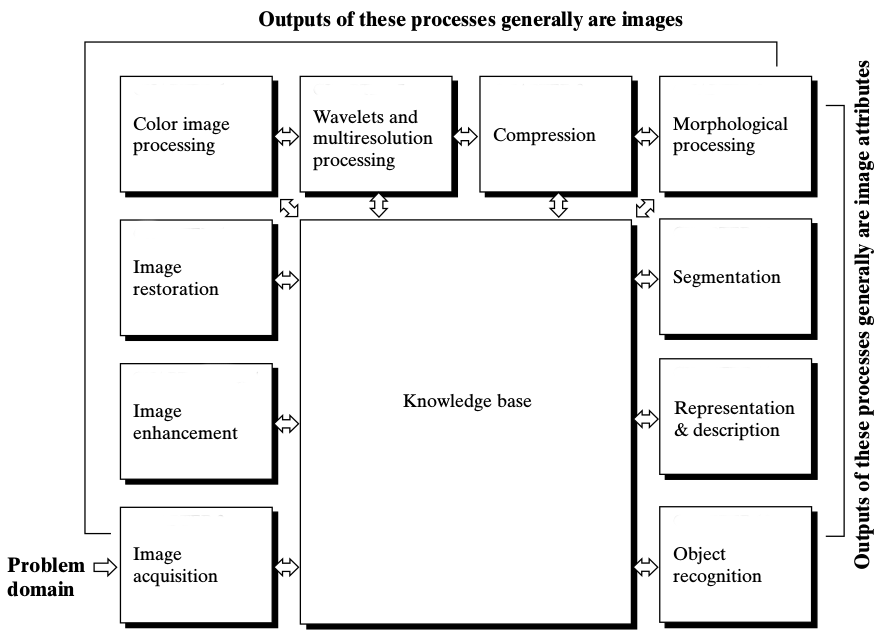
\includegraphics[scale=.5]{pics/steps.png}
    \caption{Pengeolahan citra untuk pengenalan obyek \cite{Gonzalez}}
    \label{fig:targetProcessing}
  \end{center}
\end{figure}

\section{Sub modul I/O}
Penjelasan tentang pengolahan citra berbasis \texttt{scikit-image} akan dimulai dengan sub module I/O (\textit{Input}/\textit{Output}). Pengguna harus memahami cara \texttt{scikit-image} membaca sebuah citra dan representasi dari pembacaan tersebut dalam komputer. Sebagai ilustrasi, citra uji berupa hewan \textit{baboon} \footnote{\url{https://homepages.cae.wisc.edu/~ece533/images/baboon.png}} ditunjukkan pada \figurename~\ref{fig:baboon}. 

\begin{figure}[h!]
  \begin{center}
    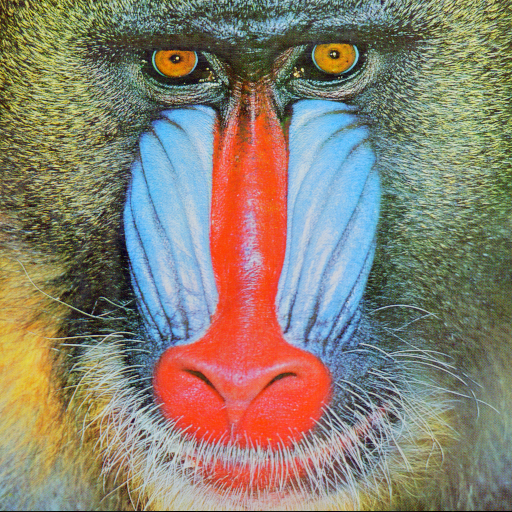
\includegraphics{pics/baboon.png}
    \caption{Citra uji \textit{baboon}}
    \label{fig:baboon}
  \end{center}
\end{figure}

\figurename~\ref{fig:baboon} berukuran \texttt{512x512} piksel yang berarti akan ada 3 matriks berukuran \texttt{512x512}, masing-masing untuk warna merah, hijau dan biru. Setiap elemen matriks akan bernilai integer di antara \texttt{0} dan \texttt{255}. Untuk membaca citra digital, digunakan fungsi \texttt{imread}, sebuah fungsi yang terdefinisi di bawah sub modul \texttt{scikit-image/io}. Masukkan perintah \lstlistingname~\ref{lst:imread} berikut di Python \texttt{shell} seperti \figurename~\ref{fig:siap}. 

\scriptsize
\begin{lstlisting}[language=python, numbers=left, numberstyle=\tiny, caption=Membaca/membuka citra, showstringspaces=false, label=lst:imread]
>>> from skimage import io
>>> img=io.imread('baboon.png')
>>> type(img)
<class 'numpy.ndarray'>
>>> img.shape
(512, 512, 3)
>>> img2=io.imread('baboon.png', True)
>>> img2.shape
(512, 512)
>>> io.imsave('baboonGS.png', img2)

\end{lstlisting}
\normalsize

Perintah di baris ke-1 menunjukkan cara untuk meng-\textit{import} pustaka \texttt{io}. Di sistem operasi Windows\textregistered, lokasi pustakanya ditunjukkan di \figurename~\ref{fig:install1}. Sedangkan di sistem operasi GNU-Linux, lokasi pustakanya berada di \texttt{/home/arya/.local/lib/python3.6/site-packages/skimage}. Di bawahnya, terdapat struktur directory seperti ditunjukkan \figurename~\ref{fig:libLocation}. Terlihat bahwa \texttt{io} adalah \textit{sub directory} yang membuat cara pemanggilan pustaka adalah seperti baris ke-1 pada \lstlistingname~\ref{lst:imread}. Cara lainnya adalah dengan mengganti perintah di baris ke-1 dengan \texttt{import skimage.io}. \textit{Directory} seperti yang ditunjukkan \figurename~\ref{fig:libLocation} sama dengan daftar sub modul dari pustaka \texttt{scikit-image}\footnote{\url{https://scikit-image.org/docs/stable/api/api.html}}. Karenanya, pola pemanggilan pustaka juga memiliki pola yang sama dengan \texttt{io}.

\begin{figure}[h!]
  \begin{center}
    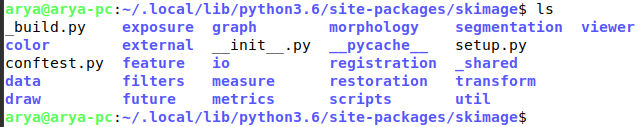
\includegraphics[scale=.65]{pics/libLocation.png}
    \caption{Berkas yang berada di dalam \textit{directory} \texttt{skimage}}
    \label{fig:libLocation}
  \end{center}
\end{figure}

Untuk baris ke-2 \lstlistingname~\ref{lst:imread}, ditunjukkan cara untuk menggunakan fungsi \texttt{imread}. Karena pustaka \texttt{io} di-\textit{import} menggunakan perintah \texttt{from skimage import io}, maka fungsi \texttt{imread} digunakan seperti pada baris ke-2. Jika pustaka \texttt{io} di-\textit{import} dengan perintah \texttt{import skimage.io}, maka fungsi \texttt{imread} digunakan dengan perintah \texttt{img=skimage.io.imread('baboon.png')}. Perlu diperhatikan, cara pembacaan citra seperti baris ke-2 hanya untuk kondisi di mana citra \texttt{baboon.png} berada pada \textit{directory} yang sama dengan lokasi Python \texttt{shell} dipanggil. Variabel \texttt{img} pada baris ke-2 menunjukkan pointer ke citra yang dibaca.

Jenis data dari variabel \texttt{img} diketahui dengan cara seperti ditunjukkan pada baris ke-3. Terlihat bahwa \texttt{img} merupakan variabel \texttt{numpy array}. Sedangkan untuk mengetahui ukuran dari \texttt{numpy array} digunakan perintah pada baris ke-5. Terlihat bahwa variabel \texttt{img} adalah 3 buah matriks berdimensi dua berukuran \texttt{512x512}. Hal ini menunjukkan bahwa citra yang sedang dibaca terdiri dari 3 komponen warna, masing-masing adalah R (\textit{Red}), G (\textit{Green}), dan B (\textit{Blue}). 

Untuk mengakses komponen warna tertentu (merah, hijau atau biru), gunakan perintah \texttt{img[:,:,0]} untuk komponen warna merah serta \texttt{img[:,:,1]} dan \texttt{img[:,:,2]} masing untuk komponen warna hijau dan biru. Pola akses matriksnya sama dengan apa yang dilakukan pada Matlab\textregistered.

Untuk membaca citra dalam bentuk skala keabuan, berikan perintah seperti baris ke-7. Baris ke-9 menunjukkan bahwa citra yang dibaca telah dikonversi ke dalam skala keabuan sehingga hanya terdiri dari 1 matriks berukuran \texttt{512x512}.

Untuk menyimpan citra yang tadi dibaca dalam bentuk skala keabuan, dapat digunakan perintah di baris ke-10. Argumen pertama (\texttt{'baboonGS.png'}) adalah nama berkas citra yang akan disimpan, sedangkan argumen kedua (\texttt{img2}) adalah matriks citra dalam skala keabuan. Hasilnya ditunjukkan pada \figurename~\ref{fig:baboonGS}.

\begin{figure}[h!]
  \begin{center}
    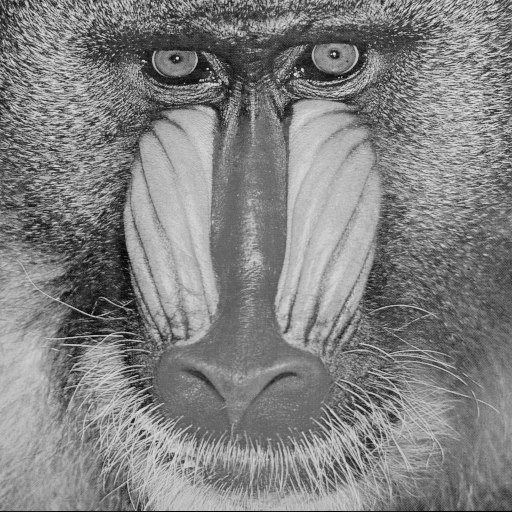
\includegraphics[scale=.125]{pics/baboonGS.png}
    \caption{Citra skala keabuan}
    \label{fig:baboonGS}
  \end{center}
\end{figure}

Sampai di sini, pustaka \texttt{numpy} tidak dibahas secara detil. Bagi yang tertarik dapat mempelajarinya secara daring di alamat \url{https://numpy.org/}. Untuk melihat fungsi apa saja yang dapat dilakukan oleh obyek \texttt{numpy} dapat diketahui dengan memberikan perintah \texttt{dir(img)} di Python \texttt{shell}, dengan \texttt{img} adalah obyek dari kelas \texttt{numpy}. 
